\documentclass[sigconf, nonacm]{acmart}
\usepackage{booktabs}
\usepackage{array}
\usepackage{float}
\usepackage{graphicx}
\usepackage{tikz}
\usetikzlibrary{arrows.meta,positioning,fit,shapes.geometric,calc,backgrounds}
\usepackage{placeins}
\usepackage{amsmath,amsthm}
\usepackage{stmaryrd}
\usepackage{enumitem}
\Urlmuskip=0mu plus 2mu

\definecolor{vldbInk}{RGB}{28,31,35}
\definecolor{vldbBlue}{RGB}{38,86,132}
\definecolor{vldbTeal}{RGB}{37,124,116}
\definecolor{vldbGold}{RGB}{154,111,43}
\definecolor{vldbRose}{RGB}{151,73,82}
\definecolor{vldbViolet}{RGB}{87,82,141}
\definecolor{vldbMist}{RGB}{239,245,248}
\definecolor{vldbMint}{RGB}{237,247,244}
\definecolor{vldbWarm}{RGB}{248,244,235}
\definecolor{vldbRule}{RGB}{190,197,201}
\definecolor{vldbGray}{RGB}{96,105,113}
\definecolor{vldbSoft}{RGB}{246,248,250}

\tikzset{
  vtitle/.style={font=\rmfamily\bfseries\fontsize{8.8}{9.6}\selectfont,
    text=vldbInk, align=center, inner sep=.4pt, text height=1.65ex,
    text depth=.30ex},
  vhead/.style={font=\rmfamily\bfseries\fontsize{7.4}{8.2}\selectfont,
    text=vldbInk, align=center, inner sep=.5pt, text height=1.55ex,
    text depth=.30ex},
  vbody/.style={font=\rmfamily\fontsize{6.9}{7.6}\selectfont,
    text=black!68, align=center, inner xsep=2.0pt, inner ysep=1.0pt,
    text height=1.50ex, text depth=.28ex},
  vsmall/.style={font=\rmfamily\fontsize{6.5}{7.1}\selectfont,
    text=black!60, align=center, inner sep=.4pt, text height=1.45ex,
    text depth=.25ex},
  vpanel/.style={rounded corners=2.5pt, line width=.52pt},
  vflow/.style={-{Latex[length=1.8mm]}, line width=.74pt,
    draw=black!52, line cap=round, line join=round}
}

\newtheorem{definition}{Definition}
\newtheorem{theorem}{Theorem}
\newtheorem{lemma}{Lemma}


\newcommand\vldbdoi{XX.XX/XXX.XX}
\newcommand\vldbpages{XXX-XXX}
\newcommand\vldbvolume{20}
\newcommand\vldbissue{1}
\newcommand\vldbyear{2027}
\newcommand\vldbauthors{\authors}
\newcommand\vldbtitle{\shorttitle}
\newcommand\vldbavailabilityurl{https://doi.org/10.5281/zenodo.21092812}
\newcommand\vldbpagestyle{plain}

\title{OptSem-C: Public Optimizer Contracts for Query Engine Portability}

\author{Haoyi Zhang}
\orcid{0009-0009-3693-786X}
\affiliation{%
  \institution{Xi'an Jiaotong-Liverpool University}
  \city{Suzhou}
  \country{China}
}
\email{hyeliozhang@gmail.com}

\author{Huaijin Ran}
\orcid{0009-0009-2482-2344}
\affiliation{%
  \institution{Nanyang Technological University}
  \city{Singapore}
  \country{Singapore}
}
\email{huaijin003@e.ntu.edu.sg}

\begin{document}
\begin{abstract}
Optimizer-behavior comparisons can fail before a performance number is measured: the comparison denominator is often a coarse vocabulary rather than an exact public contract.  Engine-selection, migration, and performance-debugging studies often compare labels such as \texttt{pushdown}, \texttt{join}, or \texttt{cost-based}.  Such labels can collapse local rewrites, source delegation, service-side stages, and runtime decisions into the same apparent capability, causing a study to compare different query-processing phenomena.

This paper presents OptSem-C, an executable benchmark and projection calculus for public optimizer behavior contracts.  A contract rule is a guarded statement over query features with explicit public modality, operator, action variant, optimizer layer, execution placement, decision time, observability, version, and public evidence.  The semantics separates behavioral worlds from evidential support, defines a conflict-aware state join, and treats lossy comparison as a projection kernel over exact contract signatures.  OptSem-C lets a study publish the vocabulary it preserves, the equivalences it assumes, and the repair fields needed to make those assumptions safe.

On a source-linked corpus spanning seven analytical SQL engines, OptSem-C shows that the failure is common and repairable.  Keyword and operator-only vocabularies declare thousands of engine--probe equivalences; 254 and 238 of those equivalences, respectively, are contradicted by exact public contracts.  The witnesses are not a formatting effect: they survive source removal, probe-family holdouts, engine-family stress, and visible-plan validation on executable SQL probes.  The missing distinctions are small and interpretable.  Placement repairs keyword collisions, optimizer layer repairs operator-only collisions, and the layer+placement basis separates all 498 headline witnesses across keyword, operator-only, and yes/no projections.  OptSem-C turns optimizer-contract comparison from an informal feature checklist into a finite, auditable query-processing relation.
\end{abstract}

\maketitle

%%% do not modify the following VLDB block %%
%%% VLDB block start %%%
\pagestyle{\vldbpagestyle}
\begingroup\small\noindent\raggedright\textbf{PVLDB Reference Format:}\\
\vldbauthors. \vldbtitle. PVLDB, \vldbvolume(\vldbissue): \vldbpages, \vldbyear.\\
\href{https://doi.org/\vldbdoi}{doi:\vldbdoi}
\endgroup
\begingroup
\renewcommand\thefootnote{}\footnote{\noindent
This work is licensed under the Creative Commons BY-NC-ND 4.0 International License. Visit \url{https://creativecommons.org/licenses/by-nc-nd/4.0/} to view a copy of this license. For any use beyond those covered by this license, obtain permission by emailing \href{mailto:info@vldb.org}{info@vldb.org}. Copyright is held by the owner/author(s). Publication rights licensed to the VLDB Endowment. \\
\raggedright Proceedings of the VLDB Endowment, Vol. \vldbvolume, No. \vldbissue\ %
ISSN 2150-8097. \\
\href{https://doi.org/\vldbdoi}{doi:\vldbdoi} \\
}\addtocounter{footnote}{-1}\endgroup
%%% VLDB block end %%%

%%% do not modify the following VLDB block %%
%%% VLDB block start %%%
\ifdefempty{\vldbavailabilityurl}{}{
\vspace{.3cm}
\begingroup\small\noindent\raggedright\textbf{PVLDB Availability Statement:}\\
The source code, data, and/or other artifacts have been made available at \url{\vldbavailabilityurl}.
\endgroup
}
%%% VLDB block end %%%

\section{Introduction}
SQL deliberately hides physical execution choices.  That abstraction is right for applications, but it becomes dangerous when the hidden choice is the object being compared in a database study.  A benchmark author may ask whether two engines support pushdown, a system integrator may compare the evidence available in plan output, and a database researcher may group systems by join or adaptivity labels.  The same SQL query can then expose different public behavior: a local predicate rewrite, connector-side execution, a service-stage graph, a runtime filter, or only a logical explanation.  Before any latency or plan-quality number is interpreted, the comparison needs to know whether those public query-processing behaviors are being treated as the same object.

The problem is easiest to see in a concrete audited case.  For probe P0009, a keyword view equates four source records under a pushdown/explain label: BigQuery federated filter delegation, BigQuery query-stage evidence, Trino connector pushdown, and Trino runtime dynamic filtering.  The public contracts do not say the same thing: they distinguish connector-source delegation, service-stage evidence, aggregate/projection pushdown, and runtime filtering.  A paper that keeps only the keywords has not found an optimizer bug; it has lost the denominator needed to decide whether two public claims were comparable in the first place.

This is not a straw-man vocabulary.  We audit 26 public comparison surfaces drawn from engine documentation, plan interfaces, and optimizer-control descriptions.  All expose keyword-style or operator-family labels, twelve expose yes/no-style controls, and none exposes the full reference payload used by OptSem-C.  The work therefore asks a narrow systems question: when public optimizer behavior is summarized at the vocabulary level exposed by comparison surfaces, which source-supported distinctions disappear, and which retained fields make the comparison auditable again?

Database research already has precise abstractions for the objects it chooses to study.  Relational semantics starts from Codd's model~\cite{codd1970relational}; Selinger-style optimizers separate access-path search from costing~\cite{selinger1979access}; Volcano exposes rule-driven and parallel query processing~\cite{graefe1990volcano}; the Volcano optimizer-generator account makes extensible search explicit~\cite{graefe1993volcano}; and Cascades turns that line into a task-driven framework~\cite{graefe1995cascades}.  Chaudhuri surveys optimizer architecture~\cite{chaudhuri1998overview}; Ioannidis surveys cost and cardinality assumptions~\cite{ioannidis1996query}; and Steinbrunn et al. study join-order search heuristics~\cite{steinbrunn1997heuristic}.  Public optimizer behavior is usually compared with much coarser vocabularies.  A cell labeled ``pushdown'' may mean predicate movement inside the engine, partition pruning, aggregation delegation, join delegation, limit delegation, or runtime filtering.  A cell labeled ``join'' may refer to a logical operator, an estimated physical operator, a distributed exchange, or a runtime profile entry.  A claim that two engines are ``cost based'' may hide whether statistics are local, connector-provided, unavailable, or revised during execution.  These shortcuts are not harmless summarization: they can create projection-induced contract collisions (a coarse vocabulary declares equality among public contracts whose reference signatures differ).

OptSem-C treats this precision problem as a query-processing systems problem, not as prose cleanup.  A \emph{public optimizer contract} is the optimizer behavior an engine exposes through plan interfaces, tuning surfaces, and system descriptions.  A source record can support a contract that is not visible in a particular textual plan, and a plan tag can expose behavior without proving the private cost model.  The object is therefore not a hidden implementation trace and not a latency measurement.  OptSem-C represents each public statement as a guarded contract rule over query features.  The rule records the action, the guard under which it applies, where the action is placed, which optimizer layer owns it, when the decision is made, how the behavior is observable, and whether the public contract requires, permits, forbids, or does not specify the action.

\textbf{Research questions.}  We ask four finite, auditable questions.  RQ1 asks whether public optimizer claims can be encoded as source-linked contracts and executable probes without becoming a latency benchmark.  RQ2 asks how often comparison vocabularies that appear in public feature claims collapse distinct source-supported contracts.  RQ3 asks which semantic fields eliminate those collisions, and which robustness checks delimit the repair claim.  RQ4 asks whether the projection-audit inner loop and SQL-denominator checks are cheap enough to rerun when the public source denominator changes, rather than trusted as a one-off manual inspection.

The central result is a projection-kernel account of these contract collisions.  Comparing optimizer contracts through a keyword or operator vocabulary applies a predeclared projection to reference signatures: the full public evidence payload inside the declared schema, not an oracle over private optimizer state.  If reference signatures disagree but fall into the same projected class, the projection has declared an equivalence that source-supported public signatures do not support.  Contract collisions are therefore denominator errors for the comparison itself; performance or cost measurements should be interpreted only after the compared behavior has been named.

OptSem-C turns that denominator question into a finite comparison relation with executable counter-witnesses, exact repair certificates, and negative controls.  The contract schema, source manifest, projection portfolio, motif crosswalk, and repair-field universe are frozen before witness counting; execution checks validate probes but never admit rules or choose repairs.  Layer and placement are therefore not learned explanations for the failures: they are schema dimensions inherited from optimizer architecture and federation literature, then tested in the same predeclared field universe as every other retained field.  Keyword projection declares 2,284 engine--probe equivalences: 2,030 have matching reference signatures and 254 are separated by reference signatures.  Operator-only projection declares 2,268 equivalences, including 238 collisions; the yes/no projection contributes six sparse source-supported records.  Across the three vocabularies, the total is 498 projection-witness records over four observed engine pairs and 486 distinct probes, where a record is keyed by projection, engine pair, and probe.  Restoring placement repairs keyword collisions; restoring optimizer layer repairs operator-only collisions; retaining layer and placement is one interpretable two-field repair basis for all headline records within the admitted public-contract corpus.

The robustness checks are designed to block three tempting overclaims.  First, the probe set is a rule-aware coverage benchmark, not an independent population sample, so we do not report statistical generalization beyond the frozen denominator.  Second, source-removal is an information-deletion stress rather than a new sample: keyword and operator-only remain nonzero after every single-source removal, and the audit separately records retained original witnesses and newly induced witnesses.  The sparse yes/no projection is reported as source-sensitive and stays outside the broad robustness claim.  Third, repair fields are not learned from failed engine-pair transfer: the reported layer-and-placement basis resolves feature-family and engine-family stress splits, while point-learned engine-pair repairs fail on held-out pairs and remain a boundary.  A field-only stress test over all 256 retained-field vocabularies leaves only 44 unsafe regions, all covered by concrete counter-witnesses; after excluding action-variant identifiers, no singleton semantic field is safe.

We also introduce OptSemBench-C, a covering benchmark for optimizer-contract behavior.  Its denominator is not raw query count.  It is coverage of optimizer-relevant feature interactions: source boundary, connector capability, join shape, predicate class, aggregation, statistics need, reuse, distribution, adaptivity, and control surface.  The generated probes are executable SQL representatives.  The probe space is then cross-checked against DPccp-style join enumeration~\cite{moerkotte2006dpccp}, JOB optimizer evidence~\cite{leis2015good}, later JOB diagnostics~\cite{leis2018looking}, exact-cardinality testing~\cite{chaudhuri2009exact}, progressive optimization~\cite{markl2004progressive}, mid-query reoptimization~\cite{kabra1998reoptimization}, adaptive query processing~\cite{deshpande2007adaptive}, and eddies~\cite{avnur2000eddies}.  We use this audit as a published-motif vocabulary stress test: 90 optimizer-motif requirements are covered by 71 distinct generated SQL representatives, so the check is concrete without pretending that generated representatives are copied JOB, TPC-H, or TPC-DS workloads.

\textbf{Contributions.} C1 defines a public optimizer contract as a query-processing object separate from SQL result equivalence and runtime performance; Section~\ref{sec:model} gives the guarded rule model and the state-join semantics.  C2 turns comparison validity into a finite projection audit: reference signatures define the public evidence relation, projected signatures expose counter-witnesses, and repair certificates identify fields that make a vocabulary safe.  C3 contributes OptSemBench-C as a denominator design for optimizer-contract comparisons across seven analytical SQL engines; Section~\ref{sec:benchcorpus} reports source-linked admission, executable probes, external-motif coverage, and zero-failure admission checks.  C4 reports the projection kernels, anti-overfitting checks, resource profile, and repair certificates: 498 headline projection-witness records, layer and placement as an interpretable repair basis for those records, and cloud replay evidence for the comparison inner loop.

Each central claim is tied to a reproducible record rather than to prose alone.  The model section defines the state table and projection obligations; the corpus section exposes source identifiers, line spans, and digest prefixes; the evaluation tables connect SQL execution, motif coverage, collision counts, and repair certificates to regenerated outputs.  The case studies then show how those aggregate certificates change comparison judgments.

\section{Precision Loss in Optimizer Comparisons}
\label{sec:problem}
Figure~\ref{fig:projection-trap} gives the smallest example.  A feature matrix maps several public optimizer contracts into the same label.  After the mapping, behaviors with different placement, action kind, and evidence layer become indistinguishable, so a study that treats the label as equality can compare non-equivalent public optimizer behavior.  Existing benchmarks and optimizer-comparison methods standardize workloads, cardinalities, or plan-quality measurements; they do not define the equality relation over public pushdown, adaptation, or plan-evidence contracts.  OptSem-C fills that gap before a JOB-, TPC-, or engine-specific measurement is interpreted.

\begin{figure}[t]
\centering
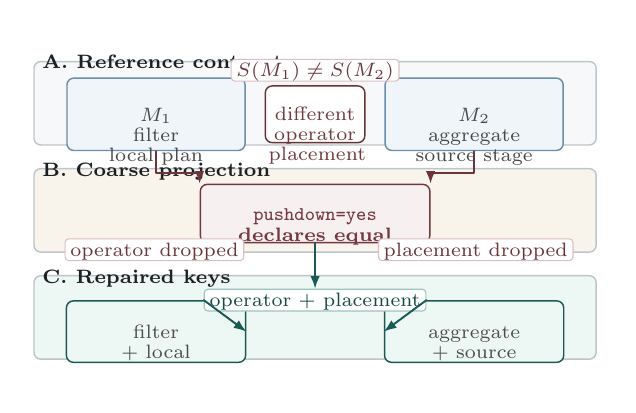
\begin{tikzpicture}[
  band/.style={vpanel, draw=vldbRule, fill=vldbSoft, minimum width=7.14cm,
    minimum height=1.06cm},
  card/.style={vpanel, draw=vldbBlue!68, fill=vldbMist, text width=2.10cm,
    minimum height=.92cm, font=\rmfamily\fontsize{6.75}{7.35}\selectfont,
    text=black!72, align=center, inner xsep=2.3pt, inner ysep=1.6pt,
    text height=1.38ex, text depth=.24ex},
  collide/.style={vpanel, draw=vldbRose!76!black, fill=vldbRose!8,
    text width=2.76cm, minimum height=.74cm,
    font=\rmfamily\bfseries\fontsize{6.95}{7.55}\selectfont,
    text=vldbRose!78!black, align=center, inner xsep=2.2pt, inner ysep=1.5pt,
    text height=1.45ex, text depth=.28ex},
  repair/.style={vpanel, draw=vldbTeal!72!black, fill=vldbMint,
    text width=2.10cm, minimum height=.78cm,
    font=\rmfamily\fontsize{6.75}{7.35}\selectfont, text=black!70,
    align=center, inner xsep=2.5pt, inner ysep=1.6pt,
    text height=1.38ex, text depth=.24ex},
  label/.style={font=\rmfamily\bfseries\fontsize{7.15}{7.85}\selectfont,
    text=vldbInk, align=left, inner sep=.3pt, text height=1.45ex,
    text depth=.28ex},
  lost/.style={vpanel, draw=vldbRose!68!black, fill=white, text width=1.18cm,
    minimum height=.72cm, font=\rmfamily\fontsize{6.60}{7.20}\selectfont,
    text=vldbRose!76!black, align=center, inner xsep=1.2pt, inner ysep=1.2pt,
    text height=1.24ex, text depth=.18ex},
  chip/.style={rounded corners=1.3pt, draw=black!14, fill=white,
    font=\rmfamily\fontsize{6.65}{7.25}\selectfont, text=vldbGray,
    inner xsep=1.9pt, inner ysep=.55pt, text height=1.32ex,
    text depth=.25ex},
  flow/.style={-{Latex[length=1.6mm]}, line width=.70pt,
    draw=black!48, line cap=round, line join=round}
]
\path[use as bounding box] (-.05,-4.30) rectangle (7.32,.24);

\begin{scope}[on background layer]
  \node[band] at (3.60,-.72) {};
  \node[band, fill=vldbWarm] at (3.60,-2.08) {};
  \node[band, fill=vldbMint] at (3.60,-3.44) {};
\end{scope}

\node[label, anchor=west] at (.12,-.19) {A. Reference contracts};
\node[label, anchor=west] at (.12,-1.56) {B. Coarse projection};
\node[label, anchor=west] at (.12,-2.92) {C. Repaired keys};

\node[card] (m1) at (1.58,-.86) {\textbf{$M_1$}\\filter\\local plan};
\node[card] (m2) at (5.62,-.86) {\textbf{$M_2$}\\aggregate\\source stage};
\node[lost] (diff) at (3.60,-.86) {different\\operator\\placement};
\node[chip, draw=vldbRose!35, text=vldbRose!70!black] at (3.60,-.30)
  {$S(M_1)\neq S(M_2)$};

\node[collide] (p) at (3.60,-2.12) {\texttt{pushdown=yes}\\declares equal};
\node[chip, draw=vldbRose!35, text=vldbRose!70!black] at (1.56,-2.58)
  {operator dropped};
\node[chip, draw=vldbRose!35, text=vldbRose!70!black] at (5.64,-2.58)
  {placement dropped};

\node[repair] (r1) at (1.58,-3.62) {filter\\+ local};
\node[repair] (r2) at (5.62,-3.62) {aggregate\\+ source};
\node[chip, draw=vldbTeal!45, text=vldbTeal!58!black] (key) at (3.60,-3.22)
  {operator + placement};

\draw[flow, draw=vldbRose!72!black] (m1.south) -- ++(0,-.28) -| (p.north west);
\draw[flow, draw=vldbRose!72!black] (m2.south) -- ++(0,-.28) -| (p.north east);
\draw[flow, draw=vldbTeal!72!black] (p.south) -- (key.north);
\draw[flow, draw=vldbTeal!72!black] (key.west) -- (r1.east);
\draw[flow, draw=vldbTeal!72!black] (key.east) -- (r2.west);
\end{tikzpicture}
\caption{Projection loss as a finite contract witness. Two source-backed contracts become equal under a coarse \texttt{pushdown=yes} denominator; retaining operator and placement separates the witness without adding private optimizer facts.}
\Description{Two reference contracts with different operator and placement fields collapse into a single pushdown=yes projection. Restoring operator and placement separates the contracts into distinct repaired keys.}
\label{fig:projection-trap}
\end{figure}


\textbf{Representative witness audits.}  Table~\ref{tab:cases} gives six concrete witness rows before the formal model.  Each starts from a familiar public label, names the engine pair and probe, shows the contract distinction that the label hides, and gives the comparison rewrite.  C1 is the running P0009 example; C2--C3 cover keyword join/plan evidence, C4--C5 cover operator-only plan and join rows, and C6 is the narrow yes/no boundary.  The same finite checker covers the 492 primary keyword/operator records and the six yes/no boundary records.

\begin{table}[t]
\centering
\caption{Concrete collision audits linking coarse labels to hidden contract pairs. C1 binds BigQuery federated pushdown~\cite{bigquery_federated_docs} and plan-stage evidence~\cite{bigquery_docs} to Trino pushdown~\cite{trino_pushdown_docs} and dynamic-filtering evidence~\cite{trino_dynamic_filtering_docs}.}
\label{tab:cases}
\footnotesize
\setlength{\tabcolsep}{1.6pt}
\renewcommand{\arraystretch}{1.05}
\begin{tabular}{@{}>{\raggedright\arraybackslash}p{0.24in}>{\raggedright\arraybackslash}p{1.82in}>{\raggedright\arraybackslash}p{0.74in}@{}}
\toprule
Case & Hidden contract contrast & Separating fields \\
\midrule
C1 & pushdown/explain: BigQuery delegation+stage evidence vs. Trino pushdown+dynamic filtering & \textbf{variant, placement, decision time} \\
C2 & plan evidence: PostgreSQL estimates vs. BigQuery/Snowflake stages & \textbf{observability, placement} \\
C3 & adaptive: compile-time planning vs. runtime repartition/AQE/conversion & \textbf{layer, decision time} \\
C4 & CTE: DuckDB/PostgreSQL inline, materialize, reuse, and disable guards & \textbf{variant, guard state} \\
\bottomrule
\end{tabular}
\end{table}


C1 is mechanical.  Source spans admit rules; P0009 triggers them with a remote aggregate; reference signatures differ on placement, layer, decision time, and observability; and the keyword projection maps both to \texttt{pushdown}+\texttt{explain}.  A coarse existence claim may remain, but portability or latency explanations must keep those fields.

\textbf{Feature-name collision.} A cell such as \texttt{pushdown=yes} may denote predicate movement inside an engine, partition pruning, connector-side predicate delegation, aggregation delegation, join delegation, limit pushdown, Top-N delegation, or runtime filtering.  These actions affect different operators and have different guards, placements, decision times, and observable plan effects.  Runtime and adaptivity distinctions are visible in Tukwila's adaptive integration~\cite{ives1999tukwila}, dynamic query plans~\cite{cole1994optimization}, and Spark SQL adaptive execution~\cite{armbrust2015spark}.  Rewrite and execution-layer distinctions appear in outerjoin rewrites~\cite{galindo1997outerjoin}, compiled execution~\cite{neumann2011efficient}, Calcite's adapter-centered optimizer framework~\cite{begoli2018calcite}, Orca's modular optimizer architecture~\cite{soliman2014orca}, and Dremel-style serving trees~\cite{melnik2010dremel}.  A single feature name can therefore erase exactly the fields a comparison needs.

\textbf{Operator disappearance.} A missing native plan node is not a reliable semantics.  It may indicate source delegation, logical-plan observability, rewrite, stage-level aggregation, or runtime-only visibility.  OptSem-C represents source-delegated execution as a positive contract action rather than as absence.  This matters for modern analytical systems whose public surfaces combine Snowflake-style cloud-service stages~\cite{dageville2016snowflake}, Redshift's managed warehouse architecture~\cite{gupta2015redshift}, C-Store column layout~\cite{stonebraker2005cstore}, row/column execution differences~\cite{abadi2008columnstores}, column-oriented design guidance~\cite{abadi2013columnoriented}, materialization policy~\cite{abadi2007materialization}, compression-coupled execution~\cite{abadi2006compression}, embedded DuckDB execution~\cite{raasveldt2019duckdb}, vectorized MonetDB/X100 execution~\cite{boncz2005monetdb}, HyPer's compiled in-memory engine~\cite{kemper2011hyper}, Vectorwise vectorized execution~\cite{zukowski2012vectorwise}, Hive's MapReduce warehouse layer~\cite{thusoo2009hive}, Impala's Hadoop SQL engine~\cite{kornacker2015impala}, distributed SQL services such as F1~\cite{shute2013f1}, and dataflow-style execution such as Spark RDDs~\cite{zaharia2012resilient}.

\textbf{Architecture ranking.} A local engine should not be ranked below a distributed engine merely because broadcast, shuffle, or remote-source delegation is not applicable.  Conversely, a federated or cloud engine should not be credited with local optimizer behavior when the public contract exposes delegation or service-side stages.  OptSem-C separates non-applicability, documented absence, documented optional behavior, and unspecified evidence.

\textbf{Observable contract versus hidden implementation.} The object of study is not what an engine could do internally.  It is what the public contract supports as a comparison claim.  This distinction is analogous to the separation between SQL equivalence and optimizer-contract equivalence.  Cosette proves SQL equivalences by reducing query semantics to logic~\cite{chu2017cosette}; semiring-based decision procedures give another equivalence foundation~\cite{chu2018usemiring}; and QED expands practical SQL equivalence checking~\cite{wang2024qed}.  Chandra and Merlin characterize conjunctive-query containment~\cite{chandra1977optimal}; Aho et al. characterize equivalence among relational expressions~\cite{aho1979equivalences}.  OptSem-C asks a different question: whether the public optimizer behavior being compared exposes the same evidence layers and comparison obligations.

These precision losses imply a minimum payload for comparing public optimizer behavior: guard, canonical action, modality, placement, decision time, observability, version, and provenance.  The rest of the paper formalizes this payload and measures what happens when a comparison vocabulary projects it away.

\section{Contract Semantics}
\label{sec:model}
A query probe is a SQL skeleton paired with a finite feature vector and validity constraints.  Features describe optimizer-relevant structure: join shape and type, predicate class, aggregation, order/limit behavior, source boundary, connector capability, statistics need, reuse structure, distribution trigger, adaptivity trigger, and optimizer control surface.  They are not workload-frequency estimates; they are coordinates on the public optimizer decision surface.

\begin{definition}[Public contract rule]
Let $\mathcal{A}$ be the finite domain of canonical optimizer actions.  An action records operator class, action kind, optimizer layer, execution placement, decision time, observability, and variant.  The state set $\mathbb{S}$ contains $\mathsf{MUST}$, $\mathsf{MAY}$, $\mathsf{MUST\_NOT}$, and $\mathsf{UNSPEC}$.  A public contract rule is $r=(\gamma,a,s,\nu,\epsilon)$, where $\gamma$ is a guard over query features, $a\in\mathcal{A}$, $s\in\mathbb{S}$, $\nu$ is the version or time window, and $\epsilon$ is evidence provenance.  For engine $e$, $C_e$ is the finite rule set, and $C_e(q)=\{r\in C_e\mid \gamma_r(\phi(q))=\mathsf{true}\}$ is the rule set applicable to probe $q$.
\end{definition}

The state domain has two components that feature matrices usually conflate.  Behaviorally, $\mathsf{MUST}$ requires an action, $\mathsf{MUST\_NOT}$ forbids it, and both $\mathsf{MAY}$ and $\mathsf{UNSPEC}$ leave it possible.  Evidentially, $\mathsf{MAY}$ is public support for optional behavior, while $\mathsf{UNSPEC}$ is lack of public support.  Equivalently, a state is interpreted as $(m,u,e)$: required behavior, allowed behavior, and evidence support.  This is why documented optional pushdown and undocumented implementation possibility are different public contracts.

For each engine-probe pair, OptSem-C constructs a contract map $M_{e,q}:\mathcal{A}\rightarrow\mathbb{S}$, defaulting every action to $\mathsf{UNSPEC}$.  Applicable rules update the map with a conflict-aware state join $\sqcup$.  The join strengthens unspecified actions when public evidence is found, preserves compatible stronger evidence, and reports contradictions instead of averaging them.  The evidence component follows database-provenance practice: support is explicit, inspectable, and attached to the object it justifies \cite{green2007provenance,buneman2001why,cheney2009provenance,green2011containment}.

\begin{figure*}[t]
\centering
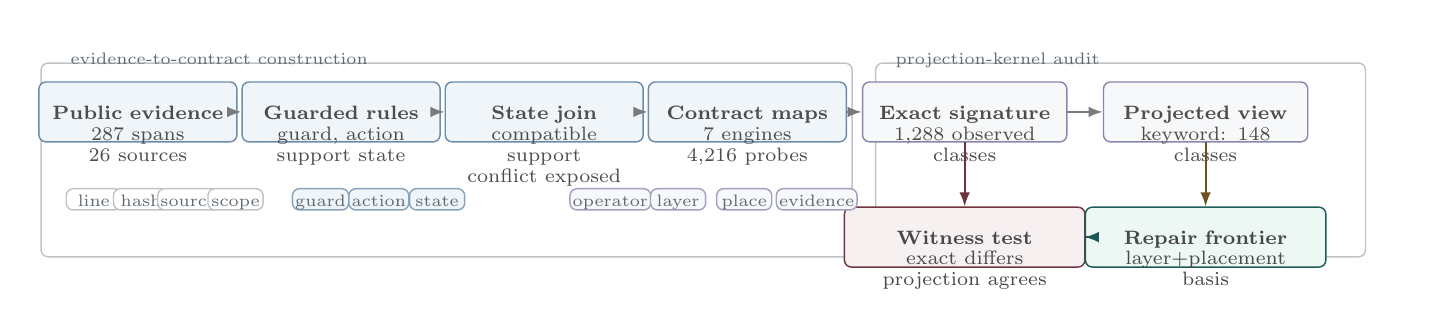
\begin{tikzpicture}[
  lane/.style={vpanel, draw=vldbRule, fill=white},
  stage/.style={vpanel, draw=vldbBlue!68, fill=vldbMist, text width=2.28cm,
    minimum height=.76cm, font=\rmfamily\fontsize{6.9}{7.6}\selectfont,
    text=black!70, align=center, text height=1.50ex, text depth=.28ex},
  sig/.style={vpanel, draw=vldbViolet!70, fill=vldbSoft, text width=2.36cm,
    minimum height=.76cm, font=\rmfamily\fontsize{6.9}{7.6}\selectfont,
    text=black!70, align=center, text height=1.50ex, text depth=.28ex},
  witness/.style={vpanel, draw=vldbRose!74!black, fill=vldbRose!8, text width=2.82cm,
    minimum height=.76cm, font=\rmfamily\fontsize{6.7}{7.4}\selectfont,
    text=black!72, align=center, text height=1.50ex, text depth=.28ex},
  repair/.style={vpanel, draw=vldbTeal!75!black, fill=vldbMint, text width=2.82cm,
    minimum height=.76cm, font=\rmfamily\fontsize{6.7}{7.4}\selectfont,
    text=black!72, align=center, text height=1.50ex, text depth=.28ex},
  chip/.style={vpanel, draw=vldbRule, fill=white, minimum width=.70cm,
    minimum height=.26cm, font=\rmfamily\fontsize{6.2}{6.8}\selectfont,
    text=vldbGray, align=center, inner xsep=1pt, inner ysep=.5pt,
    text height=1.35ex, text depth=.20ex},
  phase/.style={font=\rmfamily\fontsize{6.4}{7.0}\selectfont,
    text=vldbGray, align=center, text height=1.38ex, text depth=.22ex},
  flow/.style={vflow}
]
\path[use as bounding box] (-0.06,0.02) rectangle (17.72,3.52);

\begin{scope}[on background layer]
  \node[lane, minimum width=10.30cm, minimum height=2.46cm] at (5.26,1.84) {};
  \node[lane, minimum width=6.22cm, minimum height=2.46cm] at (13.82,1.84) {};
\end{scope}

\node[phase, anchor=west] at (.36,3.14) {evidence-to-contract construction};
\node[phase, anchor=west] at (10.84,3.14) {projection-kernel audit};

\node[stage] (evidence) at (1.34,2.45) {\textbf{Public evidence}\\287 spans\\26 sources};
\node[stage] (rule) at (3.92,2.45) {\textbf{Guarded rules}\\guard, action\\support state};
\node[stage] (join) at (6.50,2.45) {\textbf{State join}\\compatible support\\conflict exposed};
\node[stage] (map) at (9.08,2.45) {\textbf{Contract maps}\\7 engines\\4,216 probes};

\node[sig] (sig) at (11.84,2.45) {\textbf{Exact signature}\\1,288 observed\\classes};
\node[sig] (proj) at (14.90,2.45) {\textbf{Projected view}\\keyword: 148\\classes};
\node[witness] (kernel) at (11.84,.86)
  {\textbf{Witness test}\\exact differs\\projection agrees};
\node[repair] (frontier) at (14.90,.86)
  {\textbf{Repair frontier}\\layer+placement\\basis};

\node[chip] at (.78,1.34) {line};
\node[chip] at (1.38,1.34) {hash};
\node[chip] at (1.98,1.34) {source};
\node[chip] at (2.58,1.34) {scope};

\node[chip, draw=vldbBlue!55, fill=vldbMist] at (3.66,1.34) {guard};
\node[chip, draw=vldbBlue!55, fill=vldbMist] at (4.40,1.34) {action};
\node[chip, draw=vldbBlue!55, fill=vldbMist] at (5.14,1.34) {state};

\node[chip, draw=vldbViolet!55, fill=vldbSoft] at (7.34,1.34) {operator};
\node[chip, draw=vldbViolet!55, fill=vldbSoft] at (8.20,1.34) {layer};
\node[chip, draw=vldbViolet!55, fill=vldbSoft] at (9.04,1.34) {place};
\node[chip, draw=vldbViolet!55, fill=vldbSoft] at (9.96,1.34) {evidence};

\draw[flow] (evidence) -- (rule);
\draw[flow] (rule) -- (join);
\draw[flow] (join) -- (map);
\draw[flow] (map) -- (sig);
\draw[flow] (sig) -- (proj);
\draw[flow, draw=vldbRose!70!black] (sig.south) -- (kernel.north);
\draw[flow, draw=vldbGold!72!black] (proj.south) -- (frontier.north);
\draw[flow, draw=vldbTeal!72!black] (kernel) -- (frontier);
\end{tikzpicture}
\caption{Contract-comparison pipeline. Public evidence becomes guarded modal rules and exact per-engine/per-probe signatures; a projected comparison is audited by a finite witness test, and nontrivial kernels produce minimum semantic repair frontiers.}
\Description{A two-lane pipeline showing evidence spans, guarded rules, state joins, contract maps, exact signatures, projected signatures, a witness test, and a repair frontier. Small chips list the public evidence and semantic fields carried through the pipeline.}
\label{fig:contract-model}
\end{figure*}

\begin{table}[t]
\centering
\caption{Conflict-aware state join for contract support states (U=UNSPEC, N=MUST\_NOT, C=CONFLICT).}
\label{tab:state-join}
\small
\begin{tabular}{lcccc}
\toprule
$\sqcup$ & U & MAY & MUST & N \\
\midrule
U & U & MAY & MUST & N \\
MAY & MAY & MAY & MUST & C \\
MUST & MUST & MUST & MUST & C \\
N & N & C & C & N \\
\bottomrule
\end{tabular}
\end{table}


\begin{definition}[State-join algebra]
The binary operator $\sqcup$ is the partial join shown in Table~\ref{tab:state-join}.  It is total over non-conflicting pairs and returns $\mathsf{CONFLICT}$ for pairs that simultaneously require and forbid, or support and forbid, the same canonical action.  Let $x\preceq y$ denote that $x\sqcup y=y$ for non-conflicting states.  Then $\mathsf{UNSPEC}$ is the least informative state, while $\mathsf{MUST}$ and $\mathsf{MUST\_NOT}$ are incomparable incompatible commitments.
\end{definition}

\begin{lemma}[Merge invariants]
On non-conflicting states, $\sqcup$ is commutative, associative, idempotent, and monotone with respect to $\preceq$.  Therefore a contract map obtained by joining applicable rules is independent of rule order.
\end{lemma}
\begin{proof}
The properties follow by inspection of the finite table.  Idempotence holds because every diagonal entry is the input state.  Commutativity holds because the table is symmetric.  Associativity and monotonicity are checked over the finite non-conflicting triples; the only excluded triples are exactly those containing incompatible positive and negative commitments.  Lifting the pointwise operator to maps preserves the properties for every action independently.
\end{proof}

Let $W\subseteq\mathcal{A}$ be an abstract optimizer-behavior world.  A map $M$ denotes the world set
$\llbracket M\rrbracket=\{W\mid M(a)=\mathsf{MUST}\Rightarrow a\in W,\; M(a)=\mathsf{MUST\_NOT}\Rightarrow a\notin W\}$.
The evidential support set is $\mathsf{Supp}(M)=\{a\in\mathcal{A}\mid M(a)\in\{\mathsf{MUST},\mathsf{MAY},\mathsf{MUST\_NOT}\}\}$.  Behavioral containment and evidential support are intentionally separate: two maps can allow the same worlds while differing on whether an action is publicly documented.

\begin{definition}[Exact signatures, kernels, and projections]
The exact evidence-supported signature of $M$ is $S(M)=\{(a,M(a))\mid a\in\mathsf{Supp}(M)\}$.  Exact equivalence is equality of signatures over full evidence atoms.  A projection is a declared map $\pi:\mathcal{A}\times\mathbb{S}\rightarrow\mathcal{B}$ from full evidence atoms to a comparison vocabulary such as keyword, yes/no, or operator-only labels.  The projected signature is the finite image $S_\pi(M)=\{\pi(a,M(a))\mid a\in\mathsf{Supp}(M)\}$.  The projection kernel is the equivalence relation $\mathcal{K}_\pi$ where $M_i\mathcal{K}_\pi M_j$ iff $S_\pi(M_i)=S_\pi(M_j)$.  A projection-induced contract collision is a pair in $\mathcal{K}_\pi$ whose exact signatures differ.
\end{definition}

For quantitative comparison, exact compatibility is the Jaccard overlap $|S(M_i)\cap S(M_j)|/|S(M_i)\cup S(M_j)|$, and projected compatibility applies the same formula to $S_\pi$.  The denominator is evidence-supported: undocumented actions do not count as evidence of either equality or inequality.

\begin{theorem}[Finite evaluation]
For finite feature and action domains, constructing $M_{e,q}$ from finite $C_e$ and $q$ is decidable.
\end{theorem}
\begin{proof}
Every guard is a finite Boolean formula over a finite feature vector.  The applicable rule set is finite, and every applicable rule performs one lookup in the finite state-join table.  Construction therefore terminates.
\end{proof}

\begin{theorem}[Projection-kernel collision]
\label{thm:projection-kernel-loss}
For any projection $\pi$, a projection-induced contract collision is exactly the nontrivial part of the kernel $\mathcal{K}_\pi$: $M_i$ and $M_j$ collide iff $S(M_i)\ne S(M_j)$ and $M_i\mathcal{K}_\pi M_j$.  If $\pi$ is non-injective on evidence atoms, there exist contracts with such a collision witness.
\end{theorem}
\begin{proof}
The first statement unfolds the definitions: $\mathcal{K}_\pi$ is equality after projection, while exact non-equivalence is $S(M_i)\ne S(M_j)$.  For existence, take distinct evidence atoms $(a_1,s_1)\ne(a_2,s_2)$ with $\pi(a_1,s_1)=\pi(a_2,s_2)$.  Let $M_1$ contain only $(a_1,s_1)$ and $M_2$ contain only $(a_2,s_2)$.  Their exact signatures differ, but their projected signatures are the same singleton.
\end{proof}

\begin{definition}[Projection information profile]
For a finite set of observed maps $Y$, let $H(S)$ be the empirical Shannon entropy of exact signatures and $H(S_\pi)$ the entropy of projected signatures.  The entropy-retention ratio $\rho_\pi=H(S_\pi)/H(S)$ measures distinguishability retained by the comparison vocabulary.  The projected collision count is the number of projected-signature classes containing more than one exact signature class.
\end{definition}

\begin{lemma}[Kernel inflation]
If a projection declares $E_\pi$ equivalent pairs and exact comparison declares $E$ over the same pair set, then $E_\pi/E$ is the pairwise inflation factor induced by the kernel.  Every collision witness contributes to this inflation, and a zero-collision strengthened projection must have $E_\pi=E$.
\end{lemma}
\begin{proof}
Exact equivalence implies projected equivalence only when the projection is a function of the exact atom payload, so $E_\pi\ge E$.  The additional pairs counted by $E_\pi$ are exactly the unequal exact signatures that collapse under $\pi$, which are collision witnesses.  If there are none, no additional pairs are counted and the two denominators agree.
\end{proof}

\begin{theorem}[Evidence refinement]
Adding a non-conflicting evidence-backed rule cannot silently weaken a public contract: it behaviorally refines possible worlds, evidentially refines support, or both.
\end{theorem}
\begin{proof}
A $\mathsf{MUST}$ or $\mathsf{MUST\_NOT}$ rule removes worlds from $\llbracket M\rrbracket$.  A $\mathsf{MAY}$ rule may leave worlds unchanged, but changes an action from $\mathsf{UNSPEC}$ to evidence-supported.  Because the rule is non-conflicting, the state join does not erase existing support or replace a compatible stronger state with a weaker one.
\end{proof}

The remaining formal statements are a projection calculus for finite comparison audits.  They are not meant to make information loss surprising; they make the certificate obligations explicit, so Section~\ref{sec:eval} can measure which query-processing fields are empirically sufficient.  Let $F$ be the semantic-field universe and let $\pi_R$ be the repaired projection that appends the field values in $R\subseteq F$ to $\pi(a,s)$ for each evidence atom $(a,s)$.  For a finite grounded comparison set $X$, define $X_{\pi_R}=\{(M_i,M_j)\in X\mid S(M_i)\ne S(M_j)\land M_i\mathcal{K}_{\pi_R}M_j\}$.  A field set $R$ is safe, or universal, for $\pi$ on $X$ when $X_{\pi_R}=\emptyset$; otherwise it is unsafe and has a grounded counter-witness.

\begin{theorem}[Projection-lattice frontier]
\label{thm:projection-lattice}
If $R\subseteq R'\subseteq F$, then $X_{\pi_{R'}}\subseteq X_{\pi_R}$.  Consequently the safe field sets are upward closed, the unsafe field sets are downward closed, and the minimum universal repairs form an antichain frontier in the finite field lattice.
\end{theorem}
\begin{proof}
Projection $\pi_{R'}$ emits every component emitted by $\pi_R$ plus additional field values.  Adding fields can split projected equivalence classes, but cannot merge classes already separated.  Therefore any unequal pair still collapsed after adding $R'$ was also collapsed after adding $R$.  Upward closure of safe sets and downward closure of unsafe sets follow immediately, and minimal safe sets are incomparable by set inclusion.
\end{proof}

For a witness $w=(M_i,M_j)$, define its separator family $\mathcal{D}_w=\{R\subseteq F\mid M_i\not\mathcal{K}_{\pi_R} M_j\}$.  By Theorem~\ref{thm:projection-lattice}, each $\mathcal{D}_w$ is upward closed in the field lattice, and universal repair is the finite intersection problem $R\in\bigcap_{w\in X_\pi}\mathcal{D}_w$.

\begin{theorem}[Repair certificate]
\label{thm:repair-certificate}
Fix a projection $\pi$ and finite comparison set $X$.  A field set $R$ eliminates all observed collisions iff $R$ belongs to every witness separator family $\mathcal{D}_w$ for $w\in X_\pi$.
\end{theorem}
\begin{proof}
If $R\in\mathcal{D}_w$ for every witness, every pair collapsed by $\pi$ becomes separated under $\pi_R$, so $X_{\pi_R}=\emptyset$.  Conversely, if $X_{\pi_R}=\emptyset$, every original witness is separated under $\pi_R$, which is exactly membership in each separator family.
\end{proof}

\begin{theorem}[Resolution-lattice certificate]
\label{thm:resolution-lattice-certificate}
For a finite comparison set $X$ and finite field universe $F$, exhaustive enumeration of all retained-field projections over $2^{|F|}$ subsets is a complete certificate of which public optimizer fields are sufficient for safe comparison on $X$.  If a subset $R$ is unsafe, a single pair $(M_i,M_j)\in X$ with $S(M_i)\ne S(M_j)$ and $S_R(M_i)=S_R(M_j)$ is a checkable counter-certificate.  If $R$ is safe, direct equality testing over all pairs in $X$ is a checkable certificate of safety.
\end{theorem}
\begin{proof}
For each subset $R\subseteq F$, the retained-field signature $S_R$ is a deterministic projection of the exact signature.  The comparison set $X$ is finite, so checking all pairs in $X$ terminates.  Unsafety is existential and is witnessed by one collapsed unequal pair.  Safety is universal over the same finite set and is witnessed by the absence of such a pair after exhaustive enumeration.  Since every subset of $F$ is enumerated, the resulting safe and unsafe regions are complete for the chosen field universe.
\end{proof}

\begin{theorem}[Minimum repair as hitting set]
\label{thm:min-repair-complexity}
For finite semantic fields $F$ and collision witnesses $X_\pi$, deciding whether there is a universal repair of size at most $k$ is NP-complete in $|F|+|X_\pi|$.  For the fixed OptSem-C field universe, every minimum repair is exactly computable, and a certificate consists of the repaired witnesses plus counter-witnesses for every smaller field set.
\end{theorem}
\begin{proof}
Membership in NP follows by checking a candidate field set against every finite witness.  For hardness, reduce \textsc{Hitting Set}.  Given sets $H_1,\ldots,H_m\subseteq F$, create one collision witness per $H_i$ whose two contracts agree under the baseline projection and differ exactly on the fields in $H_i$.  A field set repairs that witness iff it intersects $H_i$; hence a universal repair of size $k$ exists iff the hitting-set instance has a hitting set of size $k$.  Since OptSem-C fixes a finite field universe, enumerating field subsets in increasing cardinality returns all minimum repairs.  Exhausting all smaller subsets gives the lower-bound part of the certificate.
\end{proof}

\begin{theorem}[Semantic repair basis]
Fix a finite comparison set $X$, projections $\Pi$, and a semantic field set $F$ that excludes action identifiers such as fine-grained variants.  If $R\subseteq F$ is universal for every $\pi\in\Pi$, then augmenting each projection with $R$ eliminates all observed collisions without relying on action-identifier labels.
\end{theorem}
\begin{proof}
Apply Theorem~\ref{thm:repair-certificate} to each projection independently.  Because $X$ and $\Pi$ are finite, the union of their witness sets is finite; a common $R$ that lies in every corresponding separator family leaves no collapsed unequal pair.  Excluding action identifiers restricts the admissible field universe but does not change the certificate condition.
\end{proof}

The semantics makes the comparison payload explicit.  A user comparing only operator names chooses a projection that drops placement, decision time, variant, and observability.  A feature checklist chooses an even coarser projection that can drop operator class itself.  OptSem-C does not forbid those projections; it computes exactly which kernel collisions they induce, which grounded counter-witnesses remain, and which query-processing fields repair the comparison.

\section{Benchmark and Grounded Corpus}
\label{sec:benchcorpus}
OptSemBench-C is a behavior-contract benchmark: it generates probes that cover optimizer-relevant feature interactions and measures which public contracts those probes activate.  It deliberately does not rank engines by latency.  This choice follows the benchmark principle that the metric and denominator must match the object of study.  CardEst asks whether cardinality estimates improve DBMS plan choice~\cite{han2021cardest}; CardBench stresses learned cardinality estimators in relational settings~\cite{chronis2024cardbench}; Learned Cardinalities models correlated joins~\cite{kipf2019learned}; NeuroCard models probabilistic cardinalities~\cite{yang2019neurocard}; DeepDB learns database distributions~\cite{hilprecht2020deepdb}; FactorJoin specializes join-cardinality estimation~\cite{wu2023factorjoin}; Neo learns plan choices~\cite{marcus2019neo}; and Bao evaluates learned hinting behavior~\cite{marcus2021bao}.  An optimizer-contract benchmark must instead expose semantic traps in the comparison vocabulary.

The contract schema is fixed before source extraction, witness counting, and repair search.  Its fields come from prior optimizer architecture rather than from the measured collisions.  Operator/action and layer follow System R~\cite{selinger1979access}, Volcano~\cite{graefe1990volcano}, Cascades~\cite{graefe1995cascades}, Calcite~\cite{begoli2018calcite}, and Orca~\cite{soliman2014orca}.  Placement follows Garlic federation~\cite{carey1995garlic}, BigDAWG polystores~\cite{stonebraker2015bigdawg}, Dremel serving trees~\cite{melnik2010dremel}, and Snowflake cloud execution~\cite{dageville2016snowflake}.  Decision time follows progressive optimization~\cite{markl2004progressive}, mid-query reoptimization~\cite{kabra1998reoptimization}, adaptive query processing~\cite{deshpande2007adaptive}, eddies~\cite{avnur2000eddies}, and Spark adaptive execution~\cite{armbrust2015spark}.  Observability is admitted from plan, profile, and stage evidence in the public source ledger, with provenance-style evidence separation~\cite{green2007provenance}.  Layer and placement enter the predeclared field universe; exhaustive retained-field testing later reports them as a sufficient headline repair basis, not as fields selected after seeing failures.

Let $F=F_1\times\cdots\times F_n$ be the finite feature domain and $\Psi$ the validity constraints.  A target interaction is a valid partial assignment over a feature subset.  The schema and feature domain are fixed before witness counting and derive from standard query-processing constructs and cited public optimizer surfaces, not from witnesses or motifs.  The benchmark targets global pairwise coverage plus selected three-way interactions for source boundary, connector capability, operator class, statistics need, join shape, adaptivity trigger, and distribution trigger.  The generator builds one deterministic candidate pool from renderable feature interactions and admitted public-rule guards.  It first includes 99 guard-forced completions so that every admitted rule has a reachable query shape, then greedily covers the remaining feature-interaction universe.  These two roles are reported separately: guard-forced probes prevent public contracts from becoming unreachable paper claims, while the remaining probes complete the declared feature-interaction denominator.  Neither role is treated as an independent held-out population sample.  A probe is useful when it activates a contract guard or separates two contract signatures, not when it estimates workload frequency.

\begin{observation}[Coverage]
If every valid target interaction has at least one renderable full assignment, the generator terminates with a probe set covering every renderable target interaction.
\end{observation}
\begin{proof}
The target universe is finite.  Each selected assignment covers at least one uncovered interaction.  Thus the number of uncovered interactions decreases monotonically until it reaches zero.
\end{proof}

The main empirical corpus contains only 287 source-linked grounded rules.  Each rule records a public evidence span, source URL, line range, digest, and source class.  Claims without grounded evidence, expressible guards, or public observability are outside the finite denominator rather than negative evidence.  Thus the paper claims coverage of the declared public-contract denominator, not a census of private optimizer rules.  Figure~\ref{fig:benchmark-snapshot} gives the denominator view before any collision measurement: sources, rules, probes, and motif requirements are fixed, and the zero-failure checks verify support, consistency, SQL execution, and motif coverage.  The corpus covers plan observability, pushdown, join search, distribution, materialization, runtime adaptivity, statistics, and optimizer control surfaces.  Every grounded rule is triggered by at least one generated probe, and contract merge produces no conflicts.

\begin{figure}[t]
\centering
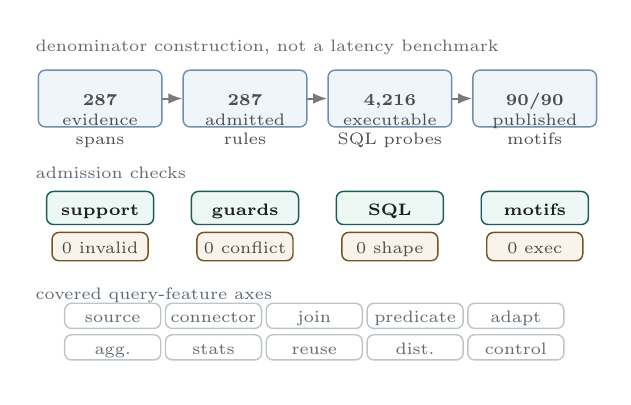
\begin{tikzpicture}[
  stage/.style={vpanel, draw=vldbBlue!66, fill=vldbMist, text width=1.50cm,
    minimum height=.72cm, font=\rmfamily\fontsize{6.45}{7.05}\selectfont,
    text=black!70, align=center, inner xsep=1pt, inner ysep=1pt,
    text height=1.48ex, text depth=.25ex},
  check/.style={vpanel, draw=vldbTeal!74!black, fill=vldbMint,
    minimum width=1.36cm, minimum height=.42cm,
    font=\rmfamily\bfseries\fontsize{6.5}{7.1}\selectfont, text=vldbInk,
    align=center, inner xsep=1pt, inner ysep=.8pt,
    text height=1.42ex, text depth=.22ex},
  axis/.style={vpanel, draw=vldbRule, fill=white, minimum width=1.22cm,
    minimum height=.32cm, font=\rmfamily\fontsize{6.2}{6.8}\selectfont,
    text=vldbGray, align=center, inner xsep=.8pt, inner ysep=.5pt,
    text height=1.35ex, text depth=.20ex},
  zero/.style={vpanel, draw=vldbGold!75!black, fill=vldbWarm,
    minimum width=1.22cm, minimum height=.36cm,
    font=\rmfamily\fontsize{6.25}{6.85}\selectfont, text=black!70,
    align=center, inner xsep=1pt, inner ysep=.8pt,
    text height=1.40ex, text depth=.22ex}
]
\path[use as bounding box] (-.06,-4.10) rectangle (7.25,.34);

\node[vsmall, anchor=west, text=vldbGray] at (.02,.13)
  {denominator construction, not a latency benchmark};
\node[stage] (ev) at (.86,-.56) {\textbf{287}\\evidence\\spans};
\node[stage] (rules) at (2.70,-.56) {\textbf{287}\\admitted\\rules};
\node[stage] (sql) at (4.54,-.56) {\textbf{4,216}\\executable\\SQL probes};
\node[stage] (motif) at (6.38,-.56) {\textbf{90/90}\\published\\motifs};
\draw[vflow] (ev) -- (rules);
\draw[vflow] (rules) -- (sql);
\draw[vflow] (sql) -- (motif);

\node[vsmall, anchor=west, text=vldbGray] at (.02,-1.48)
  {admission checks};
\node[check] at (.86,-1.95) {support};
\node[check] at (2.70,-1.95) {guards};
\node[check] at (4.54,-1.95) {SQL};
\node[check] at (6.38,-1.95) {motifs};
\node[zero] at (.86,-2.44) {0 invalid};
\node[zero] at (2.70,-2.44) {0 conflict};
\node[zero] at (4.54,-2.44) {0 shape};
\node[zero] at (6.38,-2.44) {0 exec};

\node[vsmall, anchor=west, text=vldbGray] at (.02,-3.02)
  {covered query-feature axes};
\node[axis] at (1.02,-3.32) {source};
\node[axis] at (2.30,-3.32) {connector};
\node[axis] at (3.58,-3.32) {join};
\node[axis] at (4.86,-3.32) {predicate};
\node[axis] at (6.14,-3.32) {adapt};
\node[axis] at (1.02,-3.72) {agg.};
\node[axis] at (2.30,-3.72) {stats};
\node[axis] at (3.58,-3.72) {reuse};
\node[axis] at (4.86,-3.72) {dist.};
\node[axis] at (6.14,-3.72) {control};
\end{tikzpicture}
\caption{Corpus, benchmark, and execution denominators. The same grounded denominator carries source evidence, generated probes, admission checks, and published-motif coverage.}
\Description{A compact evidence panel with four denominator counts, four admission checks, observed zero audit or execution issues, and representative covered query-feature axes.}
\label{fig:benchmark-snapshot}
\end{figure}


\begin{table*}[t]
\centering
\caption{Source-to-rule traceability for representative contracts. Each row binds a rule state/action to a public source span, digest prefix, and paraphrase used by the replay manifest.}
\label{tab:evidence-examples}
\footnotesize
\setlength{\tabcolsep}{3pt}
\begin{tabular}{@{}llp{0.15\textwidth}p{0.18\textwidth}p{0.42\textwidth}@{}}
\toprule
\multicolumn{3}{@{}l}{Contract rule} & \multicolumn{2}{l@{}}{Auditable evidence} \\
\cmidrule(r){1-3}\cmidrule(l){4-5}
Engine & State & Action & Span/digest & Source-supported paraphrase \\
\midrule
PostgreSQL~\cite{postgresql_docs} & MAY & Plan/observe/local & PG-EXPLAIN-001 bfb47e66 L46--L56 & EXPLAIN exposes estimated startup and total cost, output rows, row width, and planner-cost units. \\
BigQuery~\cite{bigquery_docs} & MAY & Exchange/adapt/cloud & BIGQUERY-PLAN-001 cc7b206a L990--L992 & The query plan may be modified during execution by adding repartition stages. \\
Snowflake~\cite{snowflake_docs} & MAY & Plan/observe/cloud & SNOWFLAKE-EXPLAIN-001 93a61359 L150--L154 & EXPLAIN compiles a statement and returns a logical execution plan rather than executing it. \\
ClickHouse~\cite{clickhouse_docs} & MAY & Join/adapt/local & CLICKHOUSE-JOINING-001 a1f757e2 L313 & With automatic join-algorithm selection, execution can switch from hash join to partial merge join. \\
DuckDB~\cite{duckdb_docs} & MAY & Materialize/inline/local & DUCK-WITH-001 2a60c8ab L482--L487 & CTE inlining is guarded by single use, absence of volatility, no grouped aggregation, and inlining hints. \\
Spark SQL~\cite{spark_docs} & MAY & Plan/adapt/distributed & SPARK-PERF-001 7e5e2b00 L129--L133 & Adaptive query execution uses runtime statistics and can re-optimize a query while it is running. \\
Trino~\cite{trino_pushdown_docs} & MUST\_NOT & Agg./pushdown/source & TRINO-PUSH-001 cc177219 L168--L176 & Aggregation pushdown does not support aggregate calls containing expressions. \\
\bottomrule
\end{tabular}
\Description{Examples of source-to-rule traceability across seven engines, including state, action, source identifier, digest prefix, line range, and paraphrased evidence.}
\end{table*}


The source set is fixed before witness counting.  We admit an engine only when public sources provide: a comparable plan or contract surface, enough detail to extract an action and applicability guard, and stable analytical-SQL behavior rather than a private vendor note.  PostgreSQL, Trino, BigQuery, Spark SQL, Snowflake, DuckDB, and ClickHouse enter through versioned source records in the evidence ledger; Calcite and DataFusion source records provide schema context rather than denominator engines.  These records are not scholarly support and not performance measurements.  They are the measured public contracts that the framework formalizes.  Proprietary workload logs, undocumented cost-model traces, future engine versions, and operator families outside the declared feature domain are excluded rather than silently counted.

The source-linked denominator spans seven engines: PostgreSQL contributes 80 admitted rules, Trino 61, BigQuery 37, Spark SQL 36, ClickHouse and Snowflake 26 each, and DuckDB 21; the largest single source supports 46 rules.  This design separates admission, probing, and execution validation.  Public sources admit rules; generated probes test guard reachability and SQL executability; DuckDB and PostgreSQL runs validate the probe denominator on two open engines, not every vendor contract.  All-engine execution would conflate SQL validity with public-contract admission.  A DuckDB source span can admit a DuckDB public contract, but a later DuckDB execution is only SQL execution and visible-plan sanity evidence; it never admits rules or chooses a repair field.  Conversely, engines without local execution still participate in collision measurements only through source-linked public contracts, source leave-one-out checks, and side-balanced witness support.

The grounded corpus is intentionally conservative.  A rule is admitted only when the evidence span supports an optimizer action, a guard or applicability condition, and an observability or placement interpretation.  Vague performance advice is excluded from the main corpus.  This policy reduces corpus size but strengthens the central claim: the evaluation is about contracts that are publicly supported, not about inferred implementation behavior.

\textbf{Contract extraction and validation checks.}  Each admitted rule records the engine, version scope, source identifier, digest, action fields, guard, and observability surface.  Human coding maps public evidence spans into the fixed schema; automated checks validate schema consistency, source linkage, guard reachability, trigger coverage, merge conflicts, SQL executability, and table-source consistency.  This is a single-extractor source-line protocol rather than formal verification or recoding agreement: every accepted row is inspectable, vague performance advice is excluded by rule, and excluded rows are outside the declared denominator.  Table~\ref{tab:evidence-examples} gives representative spans; the replay materials carry the complete rule-to-source manifest, source digests, claim-evidence graph, and regenerated table manifests.  The field schema and projection portfolio are replay inputs fixed before collision counting.  Layer plus placement is reported as an interpretable repair basis for headline witnesses after enumerating retained-field vocabularies; the frontier tables give scoped safety and do not claim global safety.  Public source records admit claims; EXPLAIN, profile, or stage surfaces bind exposed plan evidence when available; SQL execution validates the probe denominator rather than private optimizer truth.  A counted witness requires two source-supported reference signatures, projection equality under the declared vocabulary, and separation by the reported repair field.

The denominator dashboard in Table~\ref{tab:denominator-dashboard} checks that this conservatism does not create unreachable contracts or syntactic probes.  A finite-disjunction guard semantics evaluates each admitted rule against the generated probe denominator.  All 287 grounded rules have at least one triggering probe; 252 depend on query features rather than global engine labels; and no guard uses a feature dimension or value outside the benchmark domain.

\begin{table*}[t]
\centering
\caption{Denominator and validation dashboard. Bold marks complete coverage or zero observed SQL-shape/execution failures, not contract firing. The motif-cover prefix is underlined because it is the smallest human-inspection slice.}
\label{tab:denominator-dashboard}
\footnotesize
\setlength{\tabcolsep}{4pt}
\begin{tabular}{@{}llrll@{}}
\toprule
Layer & Check & Value & Scope & Interpretation \\
\midrule
Corpus & grounded rules & \textbf{287} & 26 sources & finite public-contract relation \\
Corpus & probe-supported rules & \textbf{287/287} & median support 102 & every admitted rule is triggerable \\
Corpus & non-global guards & 252 & 3 containments & query-conditional, audited overlaps \\
Guard schema & invalid dimensions & \textbf{0} & fixed feature domain & no out-of-domain guard values \\
SQL corpus & generated probes & \textbf{4,216} & digest \texttt{df107f018e37} & full executable denominator \\
SQL corpus & motif-cover prefix & \underline{48} & human inspection & compact replay slice, not cherry-picking \\
Execution & planned/executed probes & \textbf{4,216/4,216} & 91 distinct plans & every generated probe plans and runs \\
Execution & shape/exec failures & \textbf{0/0} & 18,448 rows & validation checks find no SQL-shape or runtime failures \\
Published motifs & covered requirements & \textbf{90/90} & 12 families & every declared motif has executable probe support \\
\bottomrule
\end{tabular}
\Description{A combined denominator dashboard covering grounded rules, guard checks, SQL probes, execution validation, and published motif coverage.}
\end{table*}


Coverage is reported over two denominators.  The first is benchmark coverage: every targeted renderable valid feature interaction is covered by at least one generated probe.  The second is contract triggering: every grounded rule is applicable to at least one probe.  Together these denominators make the empirical scope explicit.  A rule that cannot be triggered by any probe would indicate a benchmark gap; a feature interaction that cannot be rendered is excluded from the coverage denominator and reported as a modeling constraint.

The benchmark also exposes executable SQL shapes.  Each generated probe has a normalized SQL skeleton and shape checks for joins, filters, grouping, ordering, limits, and reuse structure.  The full 4,216-probe corpus is accompanied by a compact 48-probe motif-cover prefix.  The real-engine motif execution set uses the deterministic union of this motif cover and residual feature-axis maxima; it is not a hand-picked success set, and it is not a replacement for the full evaluation.

A common failure mode in generated benchmarks is to produce feature-complete but non-executable query text.  OptSemBench-C therefore validates every SQL skeleton on a deterministic relational catalog with local, remote, and cross-source namespaces.  This validation is not a performance baseline and is not exhaustive contract-trigger proof.  Its role is stricter and more basic: every generated probe must be parseable, plannable, executable, and shape-consistent with its feature vector.  Table~\ref{tab:denominator-dashboard} reports the validation result: all 4,216 generated probes obtain a plan and execute, with zero SQL-shape failures.  Repeating the full corpus across three deterministic catalog populations yields 12,648 successful probe-catalog executions, and DuckDB/PostgreSQL checks add 8,432 full-corpus engine--probe executions plus 142 motif-representative executions with zero execution failures.

Contract validation is layered.  Guard reachability says that each public rule has a generated probe satisfying its admitted guard; SQL execution says that the denominator is not syntactic fiction.  Visible-plan sanity checks on DuckDB and PostgreSQL expose expected plan tokens at mean rates 0.705 and 0.796 over the full corpus, and 0.756 and 0.819 on motif representatives.  These checks do not reverse-engineer private optimizers, prove every documented behavior fires on every cost-model instance, or cross-validate a source by running the same engine.  A counted witness still requires source-supported reference signatures, guard reachability, projection equality, and repair separation; runtime plan satisfaction is a separate SQL-denominator validation layer.

The same fixed probes support two budgeted evaluation orders.  The cover order is the generator's feature-interaction order.  The diagnostic order greedily maximizes newly triggered grounded rules without adding any new probe; it is a rule-coverage schedule over admitted contracts, not an unseen workload sample.  Table~\ref{tab:benchmark-efficiency} reports both.  The cover order triggers all grounded rules within 100 probes; the diagnostic order triggers 286 of 287 rules within 50 probes and all rules within 100.  Random subsets of 100 probes trigger 81\% of rules on average and 85\% at the 95th percentile.  Thus OptSemBench-C is not merely large enough to cover the surface; it also contains compact diagnostic prefixes that expose almost all grounded contracts.

\begin{table}[t]
\centering
\caption{Probe budgets for triggering grounded contract rules; random columns summarize subset baselines, with brackets giving the 5th--95th percentile interval. Bold marks complete trigger coverage.}
\label{tab:benchmark-efficiency}
\footnotesize
\begin{tabular}{rrrrr}
\toprule
Budget & Cover & Diagnostic & Random mean & Random [5,95] \\
\midrule
50 & .672 & .997 & .707 & [.627,.767] \\
100 & \textbf{1.000} & \textbf{1.000} & .811 & [.770,.850] \\
250 & \textbf{1.000} & \textbf{1.000} & .890 & [.864,.913] \\
500 & \textbf{1.000} & \textbf{1.000} & .920 & [.899,.941] \\
1000 & \textbf{1.000} & \textbf{1.000} & .951 & [.934,.969] \\
2000 & \textbf{1.000} & \textbf{1.000} & .973 & [.958,.986] \\
4216 & \textbf{1.000} & \textbf{1.000} & \textbf{1.000} & \textbf{[1.000,1.000]} \\
\bottomrule
\end{tabular}
\end{table}


A benchmark for public optimizer contracts must connect to existing database workloads without becoming another latency benchmark.  We therefore crosswalk published optimizer and benchmark motifs to OptSemBench-C feature requirements: JOB join-order sensitivity~\cite{leis2015good}, POLAR-style join structure~\cite{justen2024polar}, TPC decision-support benchmarking~\cite{poess2000tpc}, TPC-DS design~\cite{nambiar2006tpcds}, SSB~\cite{oneil2009ssb}, LDBC~\cite{erling2015ldbc}, Wisconsin~\cite{bitton1983wisconsin}, warehouse surveys~\cite{darmont2007benchmarking}, YCSB~\cite{cooper2010ycsb}, and LakeBench~\cite{deng2024lakebench}.  Figure~\ref{fig:external-motifs} reports the full executable denominator: 90 declared requirements across 12 motif families, represented by 71 distinct generated SQL probes because several queries satisfy more than one optimizer-decision requirement.  Five representative anchors illustrate the span: JOB join-order search (8/8 requirements), exact-cardinality testing (9/9), CardEst-style plan-quality sensitivity (8/8), adaptive replanning (9/9), and cross-source joinability (7/7).  Table~\ref{tab:motif-difficulty} gives the 12-family difficulty distribution.  The selected probes are feature-interaction representatives, not replacements for JOB or TPC-H queries; the crosswalk validates optimizer-decision coverage rather than workload runtime behavior.  It remains a frozen audit over optimizer-decision surfaces, not copied benchmark SQL or a latency claim; motifs outside the declared feature domain would be denominator misses.  Because motifs are checked after the schema is fixed and before repair fields are used, this is a non-circular denominator check: a counted collision still requires two source-supported signatures, projection equality, side-balanced support, and repair separation.  We claim contract-denominator adequacy and motif representation, not workload reproduction.

\begin{figure}[t]
\centering

\includegraphics[width=\columnwidth]{generated_figures/fig_external_motifs.pdf}
\caption{Published optimizer-motif denominator from the frozen table of 12 motif families and 90 requirements. A matching-probe span is the minimum--maximum number of OptSem-C probes that trigger a family; teal ranges and diamond medians keep sparse motifs visible.}
\Description{A Python-rendered log-scale range plot showing motif-family coverage and matching-probe spans for twelve optimizer and benchmark families.}
\label{fig:external-motifs}
\end{figure}

\begin{table}[t]
\centering
\caption{External motif difficulty. Matching probes are generated OptSemBench-C probes satisfying each benchmark-family motif requirement.}
\label{tab:motif-difficulty}
\scriptsize
\begin{tabular}{lrrrr}
\toprule
Suite & Motifs & Min & Median & Max  \\
\midrule
TPC-H & 8 & 1 & 87.0 & 1384  \\
TPC-DS & 8 & 86 & 164.5 & 287  \\
JOB & 8 & 55 & 87.0 & 236  \\
SSB & 6 & 89 & 101.0 & 3442  \\
CardEst & 7 & 72 & 228.0 & 259  \\
Adaptive & 6 & 72 & 205.5 & 235  \\
Federated & 8 & 72 & 91.5 & 633  \\
Controls & 8 & 70 & 72.0 & 73  \\
PostgreSQL & 8 & 72 & 73.0 & 73  \\
DuckDB & 8 & 68 & 72.0 & 364  \\
ClickHouse & 7 & 70 & 70.0 & 70  \\
Spark/Trino & 8 & 69 & 70.0 & 236  \\
\bottomrule
\end{tabular}
\Description{Motif difficulty table showing how many probes cover each external benchmark suite motif.}
\end{table}


The motif-difficulty view prevents a misleading denominator.  Some motifs are broad and match many probes, such as star-schema group-by shapes.  Others are sparse, such as a TPC-H conjunctive-filter motif that has one matching rendered probe under the current validity constraints.  Reporting both coverage and matching-probe counts makes benchmark adequacy inspectable: coverage says the motif is present, while difficulty says how concentrated or redundant that coverage is.  The executable motif suite adds a second denominator check: for each published motif, the system selects one satisfying probe and validates the generated SQL on the deterministic catalog, yielding 90 validated motif requirements, 71 distinct representatives, and 383 result rows.  Thus the motif denominator is not a list of names; it is a set of optimizer-decision requirements with concrete SQL representatives and an explicit many-to-one map.  Engine-plan validation is a separate experiment because the motif suite itself is a denominator check rather than a claim that published benchmark queries and generated probes induce identical plans.

\section{Evaluation}
\label{sec:eval}
The evaluation follows the objection path a comparison paper would face.  Do coarse public vocabularies create denominator errors?  Are counts grounded by witnesses rather than names?  Do source, probe, feature, and engine stresses preserve a finite kernel without becoming population claims?  Are projection-audit stages cheap enough to rerun when the denominator changes?  The schema, projections, source manifest, source-admission codebook, and retained-field universe are frozen before counting; exhaustive retained-field search is reported as a certificate check, while layer and placement are architecture-derived dimensions.  Execution is a post-freeze SQL-denominator consistency check: it validates probes but never admits rules or chooses fields; a non-interference check verifies that DuckDB/PostgreSQL validation files are not consumed by collision tables.  The table column ``Coll.'' is contract-level: a declared vocabulary collapses unequal public optimizer-contract signatures before any latency, plan-quality, or cost claim is interpreted.

The comparison surfaces are executable projection vocabularies and controls, not DBMS bug finders such as SQLancer~\cite{rigger2020sqlancer}, NoREC~\cite{rigger2020norec}, or other SQL fuzzing tools.  Those tools test execution behavior under generated oracles; OptSem-C audits whether a public comparison vocabulary has already collapsed unequal contracts.  Across the 26 public source surfaces, all expose keyword-style or operator-family labels, twelve expose yes/no-style controls, and none exposes the complete reference contract payload.  Reference comparison is the negative control, one-field projections are diagnostic ablations, and strengthened projections restore fields to localize missing information.  All projections are fixed before witness counting and evaluated over the same source-linked maps.  The question is how many witnesses are lost if equality is decided at that vocabulary, not whether every cited study made that exact projection.

\textbf{Coarse comparison induces concentrated, separable collisions.} The main empirical result is a finite counterexample to two coarse optimizer-comparison vocabularies, plus a positive result about narrower controls.  Table~\ref{tab:contract-collision} keeps public vocabularies, controls, stress rows, and separating fields on the same scale: keyword declares 2,284 equivalences and collapses 254 unequal reference signatures, while operator-only declares 2,268 and collapses 238.  These 11.1\% and 10.5\% fractions condition on equivalences declared by the tested vocabularies inside this corpus, not on optimizer papers.  The 492 primary records are concentrated: keyword records are BigQuery--ClickHouse (203), BigQuery--Trino (45), and ClickHouse--Trino (6); operator-only records are ClickHouse--Trino (123) and Spark SQL--Trino (115).  The remaining 17 engine pairs have zero headline collisions, so coarse labels often suffice for local-engine or non-boundary comparisons in this denominator.  The risk signal appears at cloud service, connector, distributed execution, and runtime-adaptation boundaries where public layer and placement distinctions carry the comparison.  The yes/no public-control view declares 2,036 equivalences but collapses only six, all in ClickHouse--Trino, a narrow positive result for enablement-style controls.  Primary collision pairs have reference-signature Jaccard distance 1.0 and differ by 9.09 and 5.84 evidence atoms on average.  The strict reference and strengthened surface controls have zero collapsed pairs; one-field stress rows show that a single optimizer dimension can make the denominator worse rather than safer.

\begin{table}[H]
\centering
\caption{Projection-induced contract-collision summary. Eq. is declared-equivalent engine--probe pairs; False is pairs whose exact public-contract signatures differ; Cond. is False/Eq.; Repair is the minimum separating field set.}
\label{tab:contract-collision}
\small
\begin{tabular}{lrrrl}
\toprule
Projection & Eq. & False & Cond. & Repair field(s) \\
\midrule
Keyword & 2,284 & 254 & 11.1\% & placement \\
Yes/No & 2,036 & 6 & 0.3\% & layer \\
Operator-only & 2,268 & 238 & 10.5\% & layer \\
\bottomrule
\end{tabular}
\Description{Summary table of projection-induced contract-collision counts and repair fields for keyword, yes/no, and operator-only projections.}
\end{table}


Representative witness audits appeared earlier in Table~\ref{tab:cases}; the evaluation now asks whether those examples are isolated or part of a finite kernel.

Table~\ref{tab:projection-surface-portfolio} brings the 26-row public-surface catalog into the paper.  It reports source documents that admit comparison vocabularies, not how often researchers use them.  Every admitted source exposes keyword or operator-family labels, twelve expose yes/no controls, and none exposes the full reference-signature payload.  PostgreSQL and Trino contribute 27.9\% and 21.3\% of admitted rules, while DuckDB and Snowflake contribute 7.3\% and 9.1\%; source-rich engines can create more measured opportunities, so pair counts are corpus-specific evidence rather than documentation-normalized prevalence.  If a comparison falls outside this finite catalog, the safe action is to rerun extraction rather than transfer the certificate.

\begin{table*}[t]
\centering
\caption{Projection-family synthesis over the fixed comparison set.  False-pair counts are lower-better: bold marks zero-collision controls or repairs, and underlining marks the largest unsafe family.}
\label{tab:baseline-portfolio}
\footnotesize
\setlength{\tabcolsep}{3pt}
\begin{tabular}{@{}p{2.45cm}p{3.00cm}rp{3.00cm}p{5.35cm}@{}}
\toprule
Family & Rows represented & Worst false pairs$\downarrow$ & Strongest check & Takeaway \\
\midrule
Reference controls & Exact; semantic surface & \textbf{0} & Same 88,536 comparisons & Exact equality preserves the denominator. \\
\addlinespace[1pt]
Public-label vocabularies & Keyword; yes/no; op-only & 254 & Wilson, bootstrap, leave-one-source & Public labels can be semantically unsafe. \\
\addlinespace[1pt]
One-field stress tests & Placement-only; state-only & 23,593 & Exhaustive finite audit & Single fields are not conservative. \\
\addlinespace[1pt]
Repair basis & Keyword: placement; op-only: layer; all: layer+placement & \textbf{0} & Counter-witnesses plus held-out repairs & Layer and placement resolve headline witnesses. \\
\addlinespace[1pt]
Resolution frontier & 256 subsets; 128 no-variant & \underline{59,546} & 14 minimal safe; 8 maximal unsafe & Safety is a finite frontier. \\
\bottomrule
\end{tabular}
\Description{Synthesis table grouping the projection audit into reference controls, public-label vocabularies, one-field stress tests, repair basis checks, and retained-field frontier checks.}
\end{table*}


Finite resampling keeps keyword at roughly 10--12\% and operator labels at roughly 9--12\% of corpus-specific declared equivalences.  Single-source removal is stricter to read: removing one source can delete original witnesses and create new ones, so the audit reports both nonzero counts and witness-identity movement rather than treating leave-one-source as population sampling.  The diagnosis column localizes the missing semantics: placement separates keyword, layer separates the operator row, and the strengthened semantic surface returns to zero collapsed pairs.  The sparse yes/no row is a positive boundary result for enablement-style controls: its six witnesses are all ClickHouse--Trino records and it is not used to claim broad binary-control risk.

\textbf{Projection kernels are measurable objects.} Figure~\ref{fig:projection-information} reports the finite information profile.  Reference signatures form 1,288 observed classes.  Keyword projection compresses them into 148 projected classes, retains 64\% of empirical signature entropy, and inflates declared equivalence by 12.5\%; operator-only retains more entropy but still leaves 238 pairwise collisions.  Placement-only and state-only surfaces show the opposite failure mode: a single field creates very large kernels.  The strengthened surface still has projected collisions at the signature-class level, but no pairwise collision over the engine-probe comparison set.

\begin{figure}[t]
\centering
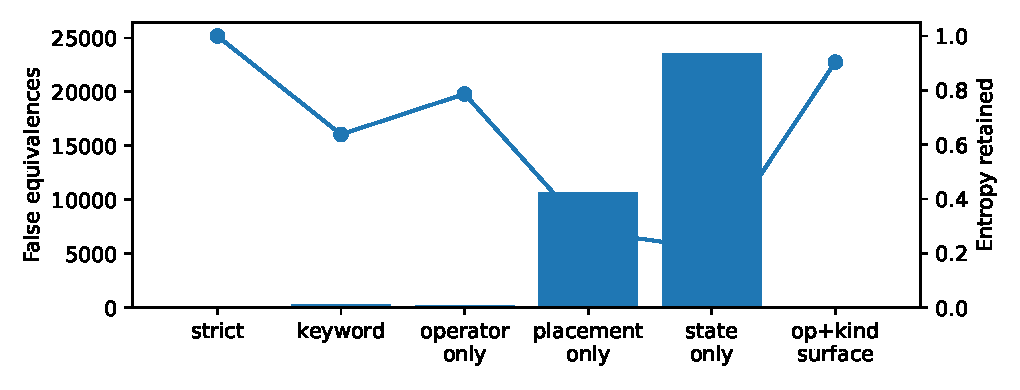
\includegraphics[width=\columnwidth]{figures/fig_projection_information.pdf}
\caption{Projection information profile. Bars show false equivalences induced by representative projections; the line shows empirical signature entropy retained by the projection.}
\Description{A bar and line chart comparing representative projections. Strict has zero false equivalences and entropy one; coarse projections lose entropy and introduce false equivalences.}
\label{fig:projection-information}
\end{figure}


\textbf{Resolution lattice stress test.}  Table~\ref{tab:resolution-lattice} enumerates all 256 retained-field subsets over the same 88,536 engine--probe comparisons.  The empty vocabulary declares 59,546 unsupported equivalences, and every singleton semantic field remains unsafe: operator leaves 238 collisions, kind 252, layer 449, and placement 10,702.  Excluding action-variant identifiers, the semantic lattice has 128 subsets, 44 unsafe regions, minimum safe field count two, 14 minimal safe vocabularies, and eight maximal unsafe vocabularies.  Ten concrete engine--probe witnesses cover all unsafe retained-field regions.

\begin{table}[t]
\centering
\caption{Exhaustive field-resolution lattice. Rows retain only the listed public optimizer fields. $|R|$ is retained fields; Classes is projected signature classes; Ent. is normalized entropy; Eq. is declared-equivalent pairs; False is unequal exact pairs still collapsed. Good rows drive False to zero with small $|R|$.}
\label{tab:resolution-lattice}
\footnotesize
\setlength{\tabcolsep}{2.5pt}
\begin{tabular}{@{}lrrrrr@{}}
\toprule
Fields & $|R|$ & Classes & Ent. & Eq. & False \\
\midrule
None & 0 & 1 & -0.000 & 61,576 & 59,546 \\
Operator & 1 & 387 & 0.787 & 2,268 & 238 \\
Action kind & 1 & 183 & 0.661 & 2,282 & 252 \\
Layer & 1 & 52 & 0.552 & 2,479 & 449 \\
Placement & 1 & 9 & 0.280 & 12,732 & 10,702 \\
Operator+layer & 2 & 591 & 0.850 & 2,030 & 0 \\
Kind+placement & 2 & 214 & 0.680 & 2,030 & 0 \\
Surface & 5 & 820 & 0.904 & 2,030 & 0 \\
All sem. & 7 & 947 & 0.934 & 2,030 & 0 \\
\bottomrule
\end{tabular}
\Description{Exhaustive field-resolution lattice table showing field count, projected classes, entropy retained, declared equivalences, and collision witnesses.}
\end{table}


The robustness view in Table~\ref{tab:robustness} checks that the headline result is not an effect of a single denominator.  The micro fraction conditions on declared equivalence; finite bands and probe-cluster resampling summarize dispersion without population inference; leave-one-source removes all rules supported by one public source.  Keyword and operator-only remain nonzero, with leave-one-source conditional-fraction ranges $[0.017,0.144]$ and $[0.032,0.148]$; the Boundary panel records retained and newly induced witnesses.

\begin{table*}[t]
\centering
\caption{Freeze, robustness, boundary, and replay dashboard. Bold zeros mark controls or separating-field surfaces; collapsed-comparison fractions are finite-corpus summaries, and source leave-one-out is an information-deletion check rather than a sampling estimate.}
\label{tab:robustness}
\footnotesize
\setlength{\tabcolsep}{3.4pt}
\begin{tabular}{@{}llrrlp{3.72cm}@{}}
\toprule
Panel & Row & Coll.$\downarrow$ & Frac./Cost & Stress & Boundary read \\
\midrule
Freeze & Denominator & -- & pre-count & SHA manifest & schema, sources, projections, replay locked \\
\midrule
Collision & Strict reference & \textbf{0} & 0.000 & control & no collapsed public signatures \\
Collision & Keyword labels & 254 & 0.111 & finite [.099,.125] & keywords hide placement \\
Collision & Operator labels & 238 & 0.105 & finite [.093,.118] & operators hide optimizer layer \\
Collision & Strengthened surface & \textbf{0} & 0.000 & separated & retained fields remove witnesses \\
\midrule
Boundary & Source LOO & -- & nonzero 26/26 & kept/new tracked & deletion check, not sampling \\
Boundary & Pair + basis & \textbf{0} & 492+6 separated & 4 pairs; 486 probes & scoped layer+placement basis \\
\midrule
Replay & Replay total & -- & 3.50 s & 455,828 input rows & excludes admission/package build \\
Replay & 8$\times$ audit lift & -- & 2.49 s & 708,288 checks/projection & inner-loop lift, not new engines \\
\bottomrule
\end{tabular}
\Description{A combined table summarizing frozen inputs, robustness, boundary checks, and replay costs. It reports finite-corpus collapsed-comparison fractions, source leave-one-out behavior, pair concentration, separation coverage, and replay timing without presenting population-level claims.}
\end{table*}


The evidence side is cross-checked without retraining on headline records: every collision has at least two public source records and side-balanced support, and the freeze manifest binds schema, sources, projections, feature-space crosswalk, implementation, and replay entrypoints before witness counting.

The Boundary panel in Table~\ref{tab:robustness} is a ledger rather than a victory table.  Keyword and operator-only remain nonzero after every leave-one-source deletion, but witness identities move: keyword retains as little as 2\% of original witnesses in the most disruptive deletion and can induce new witnesses.  Thus robustness is not witness-identity stability, and source removal is information deletion rather than a new engine-population sample.  The yes/no projection is source-sensitive and stays out of the broad robustness claim; layer+placement resolves feature-family and engine-family stress, while point-learned engine-pair bases fail on held-out pairs.

Because the 287-rule corpus is finite, the remaining checks test whether the kernel is a one-source or one-shape accident.  The 492 primary collapsed comparison records plus six yes/no boundary records occupy four observed engine pairs and 486 distinct probes, touch all 12 feature dimensions, and fully cover the value domain for 10 of them; every probe carries at most one counted witness.

\textbf{Finite-audit replay cost.}  The Replay panel in Table~\ref{tab:robustness} reports deterministic replay bounds, not stochastic performance comparisons: full audits cover 88,536 engine--probe checks per projection above 50,000 checks/s; the 8$\times$ lift repeats the relation to 708,288 checks per projection above 190,000 checks/s with prefix-scaling $R^2\geq0.98$; streaming maintenance has zero drift.

\textbf{Field certificates test an architecture hypothesis.} A certificate must match the tested projection, differ under reference contracts, separate under the proposed fields, and survive smaller-field counter-witnesses.  Placement separates keyword collisions, layer separates operator-only collisions, and layer+placement separates the 492 primary records plus the six yes/no boundary records without action-variant labels.  Other retained-field subsets can be safe for narrower projections; we report layer+placement as the uniform, architecture-readable basis that covers the headline keyword, operator-only, and yes/no families in this corpus.  This is a finite certificate, not a claim that other papers must use exactly these fields.  The hypothesis is falsifiable because operator leaves six keyword collisions, placement alone fails operator, and point-learned engine-pair bases fail held-out pairs.  Figure~\ref{fig:semantic-frontier} gives the scoped frontier; layer+placement is a counted-witness basis, not a globally safe vocabulary.

\begin{figure}[t]
\centering
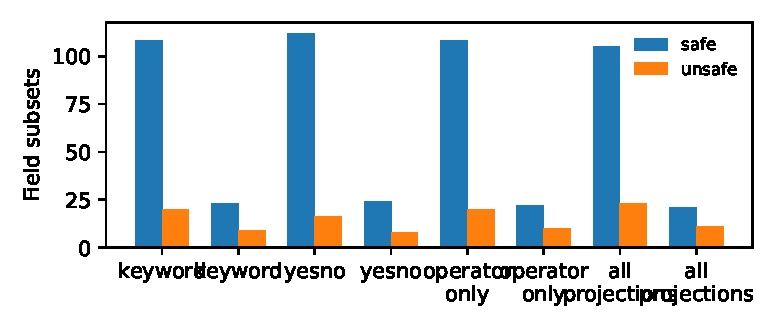
\includegraphics[width=\columnwidth]{figures/fig_semantic_frontier.pdf}
\caption{Semantic frontier over the core field lattice. Safe subsets repair all false equivalences in a scope; unsafe subsets retain a grounded counter-witness.}
\Description{A grouped bar chart comparing safe and unsafe field subsets for keyword, yes-no, operator-only, and all projections.}
\label{fig:semantic-frontier}
\end{figure}

\FloatBarrier

\section{Limitations and Conclusion}
\label{sec:conclusion}
OptSem-C is deliberately finite.  It audits a source-linked public-contract denominator, not private optimizer behavior, workload prevalence, or a population rate for database papers.  The current evidence chain is a single-extractor source-line protocol with replayable locators, digests, guards, paraphrases, downstream witnesses, and a recoding worksheet for independent follow-up; it does not claim inter-rater reliability.  DuckDB/PostgreSQL runs validate SQL constructability and visible-plan sanity for the generated denominator, not the truth of closed-source contracts.

Within that scope, the counted mechanisms are clear.  Placement separates local, delegated, distributed, and cloud execution; layer and decision time separate rewrite, planning, distribution, and runtime adaptation.  Across the 498 counted records, the ledger attributes differences to action variants (498), placement (466), layer (430), plan evidence (366), decision time (362), and operator family (281).  The practical workflow is short: name the coarse vocabulary, extract source-supported contracts, project them to the comparison table, and either retain the separating fields or state the intentionally coarse scope.  This is narrow but useful before latency or portability claims at federated SQL boundaries.
\FloatBarrier

\subsection{Concrete Collision Audits}
\label{sec:cases}
\begin{table}[t]
\centering
\caption{Concrete collision audits linking coarse labels to hidden contract pairs. C1 binds BigQuery federated pushdown~\cite{bigquery_federated_docs} and plan-stage evidence~\cite{bigquery_docs} to Trino pushdown~\cite{trino_pushdown_docs} and dynamic-filtering evidence~\cite{trino_dynamic_filtering_docs}.}
\label{tab:cases}
\footnotesize
\setlength{\tabcolsep}{1.6pt}
\renewcommand{\arraystretch}{1.05}
\begin{tabular}{@{}>{\raggedright\arraybackslash}p{0.24in}>{\raggedright\arraybackslash}p{1.82in}>{\raggedright\arraybackslash}p{0.74in}@{}}
\toprule
Case & Hidden contract contrast & Separating fields \\
\midrule
C1 & pushdown/explain: BigQuery delegation+stage evidence vs. Trino pushdown+dynamic filtering & \textbf{variant, placement, decision time} \\
C2 & plan evidence: PostgreSQL estimates vs. BigQuery/Snowflake stages & \textbf{observability, placement} \\
C3 & adaptive: compile-time planning vs. runtime repartition/AQE/conversion & \textbf{layer, decision time} \\
C4 & CTE: DuckDB/PostgreSQL inline, materialize, reuse, and disable guards & \textbf{variant, guard state} \\
\bottomrule
\end{tabular}
\end{table}


Table~\ref{tab:cases} closes the evaluation with four concrete audits from the witness ledger behind Tables~\ref{tab:contract-collision} and~\ref{tab:mechanism-hotspots}.  C1 is the running P0009 example: a coarse \texttt{pushdown}+\texttt{explain} label hides BigQuery filter delegation~\cite{bigquery_federated_docs}, BigQuery stage evidence~\cite{bigquery_docs}, Trino connector pushdown~\cite{trino_pushdown_docs}, and Trino dynamic filtering~\cite{trino_dynamic_filtering_docs}.  C2--C4 cover estimate observability, runtime adaptation, and CTE materialization; the same finite checker covers all 498 headline witnesses.

\section{Discussion and Limitations}
\label{sec:discussion}

\textbf{Optimizer interfaces as semantic interfaces.}  Public optimizer claims should name action, guard, layer, placement, decision time, and evidence surface.  These fields do not expose private cost formulas; they keep adapters, remote sources, and service stages from collapsing into one phenomenon, a boundary visible in federation~\cite{carey1995garlic} and polystores~\cite{stonebraker2015bigdawg}.

\textbf{What changes in an evaluation.}  Before ranking latency, cardinality error, or plan quality, a study can test whether compared systems share the same public contract relation.  If a pushdown table equates connector delegation with runtime filtering, the study can retain separating fields, narrow the claim, or report mixed phenomena.

\textbf{Using certificates with existing benchmarks.}  JOB, TPC-H, and TPC-DS standardize inputs and metrics, not contract equality.  A study can still execute those workloads; OptSem-C states which optimizer contracts the runs may compare and which layer, placement, or evidence surface must be separated.

\textbf{Protocol, scope, and refresh.}  Every optimizer comparison is a projection: choose a vocabulary, extract public contracts, validate the denominator, compute the kernel, and publish retained fields.  Counts are lower bounds over public evidence; later evidence becomes a source refresh.

\section{Conclusion}
OptSem-C turns coarse optimizer labels into public-evidence certificates that expose the contracts being equated, the fields needed to repair the denominator, and the counter-witnesses that break the abstraction.  Across seven analytical engines, layer, placement, decision time, observability, and action variant must be validated before performance claims are ranked.



\clearpage
\begingroup
\clubpenalty=10000
\widowpenalty=10000
\interlinepenalty=10000
\bibliographystyle{ACM-Reference-Format}
\bibliography{refs}
\endgroup
\end{document}
